%%%%%%%%%%%%%%%%%%%%%%%%%%%%%%%%%%%%%%%%%
% Programming/Coding Assignment
% LaTeX Template
%
% This template has been downloaded from:
% http://www.latextemplates.com
%
% Original author:
% Ted Pavlic (http://www.tedpavlic.com)
%
% Note:
% The \lipsum[#] commands throughout this template generate dummy text
% to fill the template out. These commands should all be removed when 
% writing assignment content.
%
% This template uses a Perl script as an example snippet of code, most other
% languages are also usable. Configure them in the "CODE INCLUSION 
% CONFIGURATION" section.
%
%%%%%%%%%%%%%%%%%%%%%%%%%%%%%%%%%%%%%%%%%

%----------------------------------------------------------------------------------------
%	PACKAGES AND OTHER DOCUMENT CONFIGURATIONS
%----------------------------------------------------------------------------------------

\documentclass{article}

\usepackage{fancyhdr} % Required for custom headers
\usepackage{lastpage} % Required to determine the last page for the footer
\usepackage{extramarks} % Required for headers and footers
\usepackage[usenames,dvipsnames]{color} % Required for custom colors
\usepackage{graphicx} % Required to insert images
\usepackage{subcaption}
\usepackage{listings} % Required for insertion of code
\usepackage{courier} % Required for the courier font
\usepackage{lipsum} % Used for inserting dummy 'Lorem ipsum' text into the template
\usepackage{hyperref} % Used for linking to websites
\usepackage{amsmath, amsthm, amssymb} % Required for writing equations
\usepackage{pythonhighlight} % Required for including Python code
\usepackage{siunitx} % Required for scientific notation

% Margins
\topmargin=-0.45in
\evensidemargin=0in
\oddsidemargin=0in
\textwidth=6.5in
\textheight=9.0in
\headsep=0.25in

\linespread{1.1} % Line spacing

% Set up the header and footer
\pagestyle{fancy}
\lhead{\hmwkFirstAuthorName, \hmwkSecondAuthorName} % Top left header
\chead{\hmwkClass\ (\hmwkClassTime): \hmwkTitle} % Top center head
%\rhead{\firstxmark} % Top right header
\lfoot{\lastxmark} % Bottom left footer
\cfoot{} % Bottom center footer
\rfoot{Page\ \thepage\ of\ \protect\pageref{LastPage}} % Bottom right footer
\renewcommand\headrulewidth{0.4pt} % Size of the header rule
\renewcommand\footrulewidth{0.4pt} % Size of the footer rule

\setlength\parindent{0pt} % Removes all indentation from paragraphs

%----------------------------------------------------------------------------------------
%	CODE INCLUSION CONFIGURATION
%----------------------------------------------------------------------------------------

\definecolor{MyDarkGreen}{rgb}{0.0,0.4,0.0} % This is the color used for comments
\lstloadlanguages{Perl} % Load Perl syntax for listings, for a list of other languages supported see: ftp://ftp.tex.ac.uk/tex-archive/macros/latex/contrib/listings/listings.pdf
\lstset{language=Perl, % Use Perl in this example
        frame=single, % Single frame around code
        basicstyle=\small\ttfamily, % Use small true type font
        keywordstyle=[1]\color{Blue}\bf, % Perl functions bold and blue
        keywordstyle=[2]\color{Purple}, % Perl function arguments purple
        keywordstyle=[3]\color{Blue}\underbar, % Custom functions underlined and blue
        identifierstyle=, % Nothing special about identifiers                                         
        commentstyle=\usefont{T1}{pcr}{m}{sl}\color{MyDarkGreen}\small, % Comments small dark green courier font
        stringstyle=\color{Purple}, % Strings are purple
        showstringspaces=false, % Don't put marks in string spaces
        tabsize=5, % 5 spaces per tab
        %
        % Put standard Perl functions not included in the default language here
        morekeywords={rand},
        %
        % Put Perl function parameters here
        morekeywords=[2]{on, off, interp},
        %
        % Put user defined functions here
        morekeywords=[3]{test},
       	%
        morecomment=[l][\color{Blue}]{...}, % Line continuation (...) like blue comment
        numbers=left, % Line numbers on left
        firstnumber=1, % Line numbers start with line 1
        numberstyle=\tiny\color{Blue}, % Line numbers are blue and small
        stepnumber=5 % Line numbers go in steps of 5
}

% Creates a new command to include a perl script, the first parameter is the filename of the script (without .pl), the second parameter is the caption
\newcommand{\perlscript}[2]{
\begin{itemize}
\item[]\lstinputlisting[caption=#2,label=#1]{#1.pl}
\end{itemize}
}

%----------------------------------------------------------------------------------------
%	DOCUMENT STRUCTURE COMMANDS
%	Skip this unless you know what you're doing
%----------------------------------------------------------------------------------------

% Header and footer for when a page split occurs within a problem environment
\newcommand{\enterProblemHeader}[1]{
%\nobreak\extramarks{#1}{#1 continued on next page\ldots}\nobreak
%\nobreak\extramarks{#1 (continued)}{#1 continued on next page\ldots}\nobreak
}

% Header and footer for when a page split occurs between problem environments
\newcommand{\exitProblemHeader}[1]{
%\nobreak\extramarks{#1 (continued)}{#1 continued on next page\ldots}\nobreak
%\nobreak\extramarks{#1}{}\nobreak
}

\setcounter{secnumdepth}{0} % Removes default section numbers
\newcounter{homeworkProblemCounter} % Creates a counter to keep track of the number of problems
\setcounter{homeworkProblemCounter}{0}

\newcommand{\homeworkProblemName}{}
\newenvironment{homeworkProblem}[1][Part \arabic{homeworkProblemCounter}]{ % Makes a new environment called homeworkProblem which takes 1 argument (custom name) but the default is "Problem #"
\stepcounter{homeworkProblemCounter} % Increase counter for number of problems
\renewcommand{\homeworkProblemName}{#1} % Assign \homeworkProblemName the name of the problem
\section{\homeworkProblemName} % Make a section in the document with the custom problem count
\enterProblemHeader{\homeworkProblemName} % Header and footer within the environment
}{
\exitProblemHeader{\homeworkProblemName} % Header and footer after the environment
}

\newcommand{\problemAnswer}[1]{ % Defines the problem answer command with the content as the only argument
\noindent\framebox[\columnwidth][c]{\begin{minipage}{0.98\columnwidth}#1\end{minipage}} % Makes the box around the problem answer and puts the content inside
}

\newcommand{\homeworkSectionName}{}
\newenvironment{homeworkSection}[1]{ % New environment for sections within homework problems, takes 1 argument - the name of the section
\renewcommand{\homeworkSectionName}{#1} % Assign \homeworkSectionName to the name of the section from the environment argument
\subsection{\homeworkSectionName} % Make a subsection with the custom name of the subsection
\enterProblemHeader{\homeworkProblemName\ [\homeworkSectionName]} % Header and footer within the environment
}{
\enterProblemHeader{\homeworkProblemName} % Header and footer after the environment
}

%----------------------------------------------------------------------------------------
%	NAME AND CLASS SECTION
%----------------------------------------------------------------------------------------

\newcommand{\hmwkTitle}{Assignment\ \#3} % Assignment title
\newcommand{\hmwkDueDate}{Monday,\ March\ 19,\ 2018} % Due date
\newcommand{\hmwkClass}{CSC411} % Course/class
\newcommand{\hmwkClassTime}{L2501} % Class/lecture time
\newcommand{\hmwkFirstAuthorName}{Chawla Dhruv} % First name
\newcommand{\hmwkSecondAuthorName}{Maham Shama Saila} % First name

%----------------------------------------------------------------------------------------
%	TITLE PAGE
%----------------------------------------------------------------------------------------

\title{
\vspace{2in}
\textmd{\textbf{\hmwkClass:\ \hmwkTitle}}\\
\normalsize\vspace{0.1in}\small{Due\ on\ \hmwkDueDate}\\
\vspace{0.1in}
\vspace{3in}
}

\author{\textbf{\hmwkFirstAuthorName, \hmwkSecondAuthorName}}
%\date{} % Insert date here if you want it to appear below your name

%----------------------------------------------------------------------------------------

\begin{document}

\maketitle
\clearpage

%----------------------------------------------------------------------------------------
%   PART 1
%----------------------------------------------------------------------------------------

\begin{homeworkProblem}

\textit{Dataset Description}\\

The dataset is present in \texttt{clean\_fake.txt} and \texttt{clean\_real.txt}. Each line of the files contains a headline all in lower case. Example: \texttt{trump warns of vote flipping on machines} is present in \texttt{clean\_fake.txt}.\\

It does seem feasible to predict whether a headline is real or fake. There are certain phrases whose presence seems to indicate if a headline is real or not:

\begin{enumerate}
    \item \texttt{clean}: appears in 1 real headline and 5 fake headlines
    \item \texttt{hillary}: appears in 24 real headlines and 150 fake headlines
    \item \texttt{donald}: appears in 832 real headlines and 231 fake headlines
\end{enumerate}

\end{homeworkProblem}
\clearpage

%----------------------------------------------------------------------------------------
%   PART 2
%----------------------------------------------------------------------------------------

\begin{homeworkProblem}

\textit{Naive Bayes Algorithm}\\

The Naive Bayes algorithm is applied on the dataset in \texttt{naive\_bayes.py}.\\

Our goal is to compute $P(fake | w)$ given $P(w | fake)$.\\

For a test headline, assume $w_i = 1$ if headline contains the word $w_i$ and $w_i = 0$ otherwise.\\

Then for training:\\
\begin{align*}
\hat{P}(w_i = 1 | fake) &= \frac {number\_of\_fake\_headlines\_containing\_w_i + m\hat{p}} {number\_of\_fake\_headlines + m}\\
\hat{P}(w_i = 0 | fake) &= 1 - \hat{P}(w_i = 1 | fake)\\
\hat{P}(w_i = 1 | real) &= \frac {number\_of\_real\_headlines\_containing\_w_i + m\hat{p}} {number\_of\_real\_headlines + m}\\
\hat{P}(w_i = 0 | real) &= 1 - \hat{P}(w_i = 1 | real)\\
\hat{P}(fake) &= \frac {number\_of\_fake\_headlines} {number\_of\_total\_headlines}\\
\hat{P}(real) &= 1 - \hat{P}(fake)\\
\end{align*}

For classifying:\\
\begin{align*}
\hat{P}(fake | w_1, w_2, ..., w_n) &\propto \hat{P}(fake) \prod_{i=1}^n \hat{P}(w_i | fake)\\
\hat{P}(real | w_1, w_2, ..., w_n) &\propto \hat{P}(real) \prod_{i=1}^n \hat{P}(w_i | real)\\
\hat{P}(fake | w_1, w_2, ..., w_n) &= \frac {\hat{P}(fake) \prod_{i=1}^n \hat{P}(w_i | fake)} {\hat{P}(fake) \prod_{i=1}^n \hat{P}(w_i | fake) + \hat{P}(real) \prod_{i=1}^n \hat{P}(w_i | real)}
\end{align*}

If $\hat{P}(fake | w_1, w_2, ..., w_n) >= 0.5$, the headline was classified as fake and otherwise, real.\\

Note: since $\prod_{i=1}^n \hat{P}(w_i | real)$ and $\prod_{i=1}^n \hat{P}(w_i | fake)$ invloves computing products of a lot of really small numbers (which might result in underflow), the property that $a_1, a_2, ..., a_n = exp(log a_1 + log a_2 + ... + log a_n)$ was used to compute the product.\\

The values of $m$ and $\hat{p}$ were determined using random search over the performance of validation set.\\

$m$ is the number of examples to be included in the prior calculation. The more number of examples, the more $\hat{p}$ influences the final probability calculation. Values of $m$ were tried on a logarithmic scale of $1, 10, 100, 1000$. Out of these, $m = 1$ gave the best result.\\

$\hat{p}$ is the prior probability of the word being real or fake. Values of $\hat{p}$ were tried in $0.1, 0.5, 0.7, 1$. Out of these $\hat{p} = 1$ gave the best performance.\\

Note: $\hat{p}$ was used as prior in calculation for both word being real and fake. This finding (low $m$ and $\hat{p}$) seems to imply that our prior assumptions in this case are not very accurate and it was best to have prior influence as minimal as possible.\\

The final results were as follows:
\begin{enumerate}
    \item Training Set: $97.28\%$
    \item Validation Set: $83.46\%$
    \item Testing Set: $85.68\%$
\end{enumerate}

\end{homeworkProblem}
\clearpage

%----------------------------------------------------------------------------------------
%   PART 3
%----------------------------------------------------------------------------------------

\begin{homeworkProblem}

\textit{Naive Bayes Algorithm: Indicative Words}\\

\textbf{Part 3(a)}

The keywords ranked according to the four different probabilities are listed in the table below.
\begin{center}
\begin{tabular}{ | l | l | l | l | }
	\hline
	$P(fake | \neg word)$  & $P(fake | word)$ & $P(real | \neg word)$ & $P(real | word)$ \\ \hline
	richardson  & powell  & pardon  & breaking  \\ \hline
	snaps  & strong & megyn  & soros  \\ \hline
	annouces & tough & buses  & 3 \\ \hline
	divides & phoenix & africa  & woman  \\ \hline
	cuba  & industry & editors  & steal  \\ \hline
	speaks  & rules & armed  & u  \\ \hline
	apprentice & care  & responsabilidad  & here  \\ \hline
	fourth  & duterte  & gutless  & m  \\ \hline
	misleading & covfefe  & khan  & reporter  \\ \hline
	magazine  & shorten  & revelation & homeless  \\ \hline
\end{tabular}
\label{tab: List of top 10 indicative words}
\end{center}

The probabilities were calculated as follows: 

\begin{equation*}
	P(class) = \frac{\text{\# of headlines of that class}}{\text{total \# of headlines}}
\end{equation*}

\begin{equation*}
	P(word | class) = \frac{\text{ \# of occurrences of word in headlines of that class}}{\text{total number of headlines of that class}}
\end{equation*}

\begin{equation*}
P(class | word) = \frac{P(word | class) * P(class)} { ( P(word|fake) * P(fake) + P(word|real) *P(real) }
\end{equation*}

\begin{align*}
	P(class | \neg word) = \frac{P(\neg word | class)P(class)}{P(\neg word)}
\end{align*}

\begin{equation*}
	P(\neg word | class) = 1 - P(word | class)
\end{equation*}
\begin{equation*}
	P(\neg word) = \frac{\text{headlines without word}}{\# \text{headlines}}
\end{equation*}

The values of $P(class|word)$ are generally much larger than those of $P(class| \neg words)$. Thus, the presence of words seem like stronger predictors of whether a headline is real or fake than absence. 

\textbf{Part 3(b)} \\
 
Since the top ten words listed do not contain any stop-words, the list remains unchanged upon removing stop words.  \\

\textbf{Part 3(c)} \\
 
Stop words are not helpful when headlines are being assessed for their content, but are important for context. For example,  the phase "trump can't think" and the phrase "trump can think" reduce to "trump think" if we remove the stop words, (cant, can). The reduced phrase tell us what the sentence is about but do not convey the original message of each sentence. 

\end{homeworkProblem}
\clearpage

%----------------------------------------------------------------------------------------
%   PART 4
%----------------------------------------------------------------------------------------

\begin{homeworkProblem}

\textit{Logistic Regression}\\

PyTorch framework was used to create a Logistic Regression model. This model is constructed and trained in \texttt{logistic\_classifier.py}. The code is reproduced below.\\

\begin{python}
# Model
class LogisticRegression(nn.Module):
    def __init__(self, input_size, num_classes):
        super(LogisticRegression, self).__init__()
        self.linear = nn.Linear(input_size, num_classes)
    
    def forward(self, x):
        out = self.linear(x)
        return out

def train_LR_model(training_set, training_label, validation_set, validation_label, total_unique_words):
    """
    Trains Logistic Regression Numpy model

    PARAMETERS
    ----------
    training_set, validation_set: numpy arrays [num_examples, total_unique_words]
        For each headline in a set:
        v[k] = 1 if kth word appears in the headline else 0

    training_label, validation_label: numpy arrays [num_examples, [0, 1] or [1, 0]]
        [0, 1] if headline is fake else [1, 0]

    total_unique_words: int
        total number of unique words in training_set, validation_set, testing_set

    RETURNS
    -------
    model: LogisticRegression instance
        fully trained Logistic Regression model

    REQUIRES
    --------
    LogisticRegression: PyTorch class defined
    """
    # Hyper Parameters 
    input_size = total_unique_words
    num_classes = 2
    num_epochs = 800
    learning_rate = 0.001
    reg_lambda = 0.01

    model = LogisticRegression(input_size, num_classes)

    x = Variable(torch.from_numpy(training_set), requires_grad=False).type(torch.FloatTensor)
    y_classes = Variable(torch.from_numpy(np.argmax(training_label, 1)), requires_grad=False).type(torch.LongTensor)

    # Loss and Optimizer
    # Softmax is internally computed.
    # Set parameters to be updated.
    loss_fn = nn.CrossEntropyLoss()  
    optimizer = torch.optim.Adam(model.parameters(), lr=learning_rate)  

    # Training the Model
    for epoch in range(num_epochs+1):
        # Forward + Backward + Optimize
        optimizer.zero_grad()
        outputs = model(x)
        l2_reg = Variable(torch.FloatTensor(1), requires_grad=True)
        for W in model.parameters():
            l2_reg = l2_reg + W.norm(2)
        loss = loss_fn(outputs, y_classes) + reg_lambda*l2_reg
        loss.backward()
        optimizer.step()
        
        if epoch % 100 == 0:
            print("Epoch: " + str(epoch))

            # Training Performance
            x_train = Variable(torch.from_numpy(training_set), requires_grad=False).type(torch.FloatTensor)
            y_pred = model(x_train).data.numpy()
            train_perf_i = (np.mean(np.argmax(y_pred, 1) == np.argmax(training_label, 1))) * 100
            print("Training Set Performance  : " + str(train_perf_i) + "%")      

            # Validation Performance  
            x_valid = Variable(torch.from_numpy(validation_set), requires_grad=False).type(torch.FloatTensor)
            y_pred = model(x_valid).data.numpy()
            valid_perf_i = (np.mean(np.argmax(y_pred, 1) == np.argmax(validation_label, 1))) * 100
            print("Validation Set Performance:  " + str(valid_perf_i) + "%\n")

    return model
\end{python}

The final results were as follows:
\begin{enumerate}
    \item Training Set: $98.46\%$
    \item Validation Set: $82.04\%$
    \item Testing Set: $84.86\%$
\end{enumerate}

The learning curves are shown in Figure 1.\\

\begin{figure*}[h!]
    \centering
    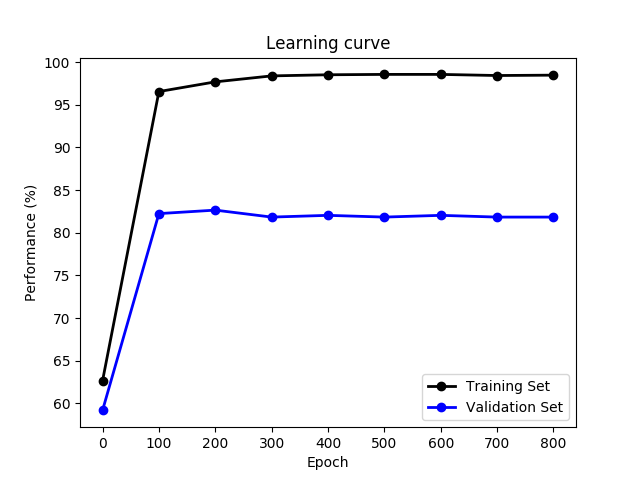
\includegraphics[scale=1]{figures/part4_learning_curve.png}
    \caption{Logistic Regression Learning Curve}
    \label{fig:fig1}
\end{figure*}

For regularization parameters, both $L1$ and $L2$ regularization were tried. $L2$ regularization performed $10\%$ better. The $\lambda$ values for $L2$ regularization was varied for values $0.001,0.001,0.05,0.01,0.1,0.5$. Out of these, $0.01$ performed the best.\\

\end{homeworkProblem}
\clearpage

%----------------------------------------------------------------------------------------
%   PART 5
%----------------------------------------------------------------------------------------

\begin{homeworkProblem}

\textit{Naive Bayes vs Logistic Regression}\\

\begin{align*}
\theta_0 + \theta_1 I_1(x) + \theta_2 I_2(x) + \hdots + \theta_k I_k(x) > thr
\end{align*}

$k$ is the total number of unique words that appear in all headlines.\\
$I_i(x)$ is equal to 1 if $x_i$ is present in the headline under consideration, 0 otherwise.\\

\textbf{Naive Bayes}\\
$\theta_i$ is equal to $log \frac {P(x_i = 1 | y = fake)} {P(x_i = 1 | y = real)} - log \frac {P(x_i = 0 | y = fake)} {P(x_i = 0 | y = real)}$\\

\textbf{Logistic Regression}\\
$\theta_i$ is equal to $max(log \frac {P(x_i = 1 | y = fake)} {P(x_i = 1 | y = real)}, log \frac {P(x_i = 0 | y = fake)} {P(x_i = 0 | y = real)})$\\

\end{homeworkProblem}
\clearpage

%----------------------------------------------------------------------------------------
%   PART 6
%----------------------------------------------------------------------------------------

\begin{homeworkProblem}

\textit{Logistic Regression: Indicative Words}\\

\textbf{Part 6(a) and 6(b)}\\

This part can be reproduced by calling \texttt{part6()}. The results are reproduced here:

\begin{verbatim}
Top 10 positive thetas (including stop-words):
1: trumps
2: tax
3: australia
4: tapping
5: says
6: debate
7: latest
8: hacking
9: business
10: asia


Top 10 negative thetas (including stop-words):
1: victory
2: breaking
3: information
4: elect
5: veterans
6: predicts
7: black
8: watch
9: d
10: won


Top 10 positive thetas (excluding stop-words):
1: trumps
2: tax
3: australia
4: tapping
5: says
6: debate
7: latest
8: hacking
9: business
10: asia


Top 10 negative thetas (excluding stop-words):
1: victory
2: breaking
3: information
4: elect
5: veterans
6: predicts
7: black
8: watch
9: d
10: won
\end{verbatim}

\texttt{Part 6(a)} does contain similar words to \texttt{Part 3(a)}. Words like \texttt{australia, business, asia} appear in \texttt{real\_under\_absence.txt} while words like \texttt{breaking, d} appear in \texttt{real\_under\_presence.txt}\\

The exlcusion of stopwords in both lists in Parts $6$ and $3$ have no effect on the top $10$ lists.\\

\textbf{Part 6(c)}\\

Using magnitude of the logistic regression parameters to indicate importance of a feature can be a bad idea in general if features are not normalized.\\

Example: for a predictor of the selling price there are two factors: land area and width of the plot. Now, generally the land area is bigger in pure magnitude compared to the width of the plot, so unless the features are normalized, land area will influence the classifier more than the plot width.\\

However, it is reasonable to use logistic regression in this problem because each feature is either 0 or 1 so no one feature carries more importance than the rest. It's akin to the features already being normalized.\\

\end{homeworkProblem}
\clearpage

%----------------------------------------------------------------------------------------
%   PART 7
%----------------------------------------------------------------------------------------

\begin{homeworkProblem}

\textit{Decision Trees}\\

\textbf{Part 7(a)}\\

The relationship between between maximum depth of the tree and the training/validation accuracy can be seen below:\\

\begin{verbatim}
Depth: 2
Training Set Accuracy  : 70.6165282029
Validation Set Accuracy: 69.1836734694


Depth: 5
Training Set Accuracy  : 73.2837778749
Validation Set Accuracy: 67.5510204082


Depth: 10
Training Set Accuracy  : 78.1810231745
Validation Set Accuracy: 69.7959183673


Depth: 20
Training Set Accuracy  : 85.5268911237
Validation Set Accuracy: 71.4285714286


Depth: 50
Training Set Accuracy  : 95.2339309139
Validation Set Accuracy: 73.4693877551


Depth: 75
Training Set Accuracy  : 97.9011805859
Validation Set Accuracy: 73.8775510204


Depth: 100
Training Set Accuracy  : 99.0380411019
Validation Set Accuracy: 73.8775510204


Depth: 150
Training Set Accuracy  : 100.0
Validation Set Accuracy: 73.8775510204


Depth: 200
Training Set Accuracy  : 100.0
Validation Set Accuracy: 72.6530612245


Depth: 500
Training Set Accuracy  : 100.0
Validation Set Accuracy: 73.2653061224
\end{verbatim}

As can be seen, with increasing depth, the performance increases at first, and then overfits.\\

The final testing accuracy (on $max\_depth = 150$ comes out to be $75.66\%$).\\

This can be reproduced by running \texttt{part7()} in \texttt{fake.py}.\\

In addition, we did not use any other parameters for which we are using non-default values, although non-default parameters were experimented with for \texttt{criterion, splitter,} and \texttt{max\_features} and their performance measured on the validation set.\\

\textbf{Part 7(b)}\\

The first two layers of the tree are visualized here:\\

\begin{figure*}[h!]
    \centering
    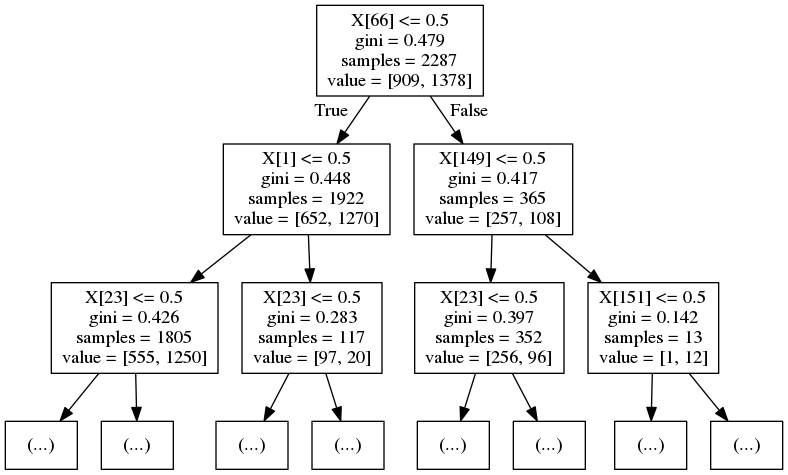
\includegraphics[scale=0.5]{figures/decision_tree.png}
    \caption{First two layers of the decision tree}
    \label{fig:fig2}
\end{figure*}

This can be reproduced by running \texttt{part7()} in \texttt{fake.py}.\\

The only important feature common between the first two levels of the decision tree visualization and Parts $3$ and $6$ seems to be the word \texttt{trumps}. The lack of common words may be attributed to the fact that NB and Logistic Regression are classifying words important to classifying headlines as real or fake whereas the decision tree is objectified towards identifying a split with highest information split on either side of tree which may not directly correspond to the word as being indicative of one class or the other.\\

\textbf{Part 7(c)}\\

\begin{center}
    \begin{tabular}{| l | l | l | l |}
        \hline
        Method & Training Set Accuracy & Validation Set Accuracy & Testing Set Accuracy \\ \hline
        Naive Bayes & $97.28\%$ & $83.46\%$ & $85.68\%$ \\ \hline
        Logistic Regression & $98.46\%$ & $82.04\%$ & $84.86\%$ \\ \hline
        Decision Tree & $100.0\%$ & $73.87\%$ & $75.66\%$ \\ \hline
    \end{tabular}
\end{center}

The performance of the three classifiers is summarized in the table above. As can be seen, Naive Bayes and Logistic Regression had similar performances, while Decision Trees had the most overfitting.\\

\end{homeworkProblem}
\clearpage

%----------------------------------------------------------------------------------------
%   PART 8
%----------------------------------------------------------------------------------------

\begin{homeworkProblem}
	
\textbf{Part 8(a)}\\
Mutual information is defined as the amount of information we learn about the value B knowing the value of A. It is given by 
$$I(A;B) = H(B) - H(B|A) = H(B) - H(A|B)$$
where
\begin{align*}
H(B|A) &= \sum_a P(A=a)H(B|A=a) \\
	   &= \sum_a P(A=a) [-\sum_bP(B=b|A=a)\log_2P(B=b|A=a) ]
\end{align*}

In our case, A = Y = $ \{real, fake \} $ and $B = X = \{ x_i="the" \} $.
$$H(Y) = -P(real) \log_2P(real) - P(fake) \log_2P(fake)$$

%also multiply by P(the) and P(not the)
%include results from Part 3

\begin{align*}H(Y|"the") &= P(real) [ -P(real|"the") \log_2P(real|"the") -P(real| \neg "the") \log_2P(real| \neg"the")]\\
			 &\hspace{0.3cm} + P(fake)[-P(fake|"the") \log_2 P(fake|"the") -P(fake|\neg "the") \log_2 P(fake| \neg "the")] 
\end{align*}


\begin{align*}
	I(Y;X) &= H(Y) - H(Y|X)  \\
		   &= H(Y) -  P(X="the")H(Y|X="the")
\end{align*}

From part3, P(real) = 0.6025, P(fake) = 0.3975, $P(real|"the")$ = 0.9901, $P(fake|"the")$ = 0.0099, $P(real|\neg "the") = 0.0933 $ , $P(fake|\neg"the") = 0.3364$ \\

\begin{align*}
	H(Y) &= - 0.6025 \log_2(0.6025) - 0.3975 \log_2(0.3975) \\ 
		 &= 0.9695
\end{align*}
\begin{align*} 
H(Y|"the") &= 0.6025[- 0.9901 \log_2(0.9901) - 0.0933 \log_2(0.0933) ]  \\
		   &\hspace{0.3cm} + 0.3975 [- 0.0099 \log_2(0.0099) - 0.3364 \log_2(0.3364) ] \\
		   &= 0.4373
\end{align*}
Thus, 
\begin{align*}
	I(Y;X) &= 0.9695 - 0.4373 \\
		   &= 0.5322
\end{align*}

\end{homeworkProblem}

\textbf{Part 8(b)}\\
Let $x_j$ = "hillary". From previous parts, $P(real|"hillary")$ = 0.9793, $P(real | \neg "hillary")$ = 0.0154, $P(fake|"hillary")$ = 0.02074, $P(fake| \neg "hillary")$ = 0.1344.  \\

\begin{align*}
H(Y) &= - 0.6025 \log_2(0.6025) - 0.3975 \log_2(0.3975) \\ 
&= 0.9695
\end{align*}

\begin{align*} 
H(Y|"hillary") &= 0.6025[ - 0.9793 \log_2(0.9793) - 0.0154 \log_2(0.01548) ]  \\
&\hspace{0.3cm} + 0.3975 [- 0.02074 \log_2(0.02074) - 0.1344 \log_2(0.1344) ] \\
&= 0.2744
\end{align*}

Thus,
\begin{align*}
I(Y;X) &= 0.9695 - 0.2744 \\
&= 0.6951
\end{align*}

The value obtained for $I(Y|x)$ in part 8(b) is larger than that obtained in part 8(a)

\clearpage

%----------------------------------------------------------------------------------------

\end{document}